\documentclass[1p]{elsarticle_modified}
%\bibliographystyle{elsarticle-num}

%\usepackage[colorlinks]{hyperref}
%\usepackage{abbrmath_seonhwa} %\Abb, \Ascr, \Acal ,\Abf, \Afrak
\usepackage{amsfonts}
\usepackage{amssymb}
\usepackage{amsmath}
\usepackage{amsthm}
\usepackage{scalefnt}
\usepackage{amsbsy}
\usepackage{kotex}
\usepackage{caption}
\usepackage{subfig}
\usepackage{color}
\usepackage{graphicx}
\usepackage{xcolor} %% white, black, red, green, blue, cyan, magenta, yellow
\usepackage{float}
\usepackage{setspace}
\usepackage{hyperref}

\usepackage{tikz}
\usetikzlibrary{arrows}

\usepackage{multirow}
\usepackage{array} % fixed length table
\usepackage{hhline}

%%%%%%%%%%%%%%%%%%%%%
\makeatletter
\renewcommand*\env@matrix[1][\arraystretch]{%
	\edef\arraystretch{#1}%
	\hskip -\arraycolsep
	\let\@ifnextchar\new@ifnextchar
	\array{*\c@MaxMatrixCols c}}
\makeatother %https://tex.stackexchange.com/questions/14071/how-can-i-increase-the-line-spacing-in-a-matrix
%%%%%%%%%%%%%%%

\usepackage[normalem]{ulem}

\newcommand{\msout}[1]{\ifmmode\text{\sout{\ensuremath{#1}}}\else\sout{#1}\fi}
%SOURCE: \msout is \stkout macro in https://tex.stackexchange.com/questions/20609/strikeout-in-math-mode

\newcommand{\cancel}[1]{
	\ifmmode
	{\color{red}\msout{#1}}
	\else
	{\color{red}\sout{#1}}
	\fi
}

\newcommand{\add}[1]{
	{\color{blue}\uwave{#1}}
}

\newcommand{\replace}[2]{
	\ifmmode
	{\color{red}\msout{#1}}{\color{blue}\uwave{#2}}
	\else
	{\color{red}\sout{#1}}{\color{blue}\uwave{#2}}
	\fi
}

\newcommand{\Sol}{\mathcal{S}} %segment
\newcommand{\D}{D} %diagram
\newcommand{\A}{\mathcal{A}} %arc


%%%%%%%%%%%%%%%%%%%%%%%%%%%%%5 test

\def\sl{\operatorname{\textup{SL}}(2,\Cbb)}
\def\psl{\operatorname{\textup{PSL}}(2,\Cbb)}
\def\quan{\mkern 1mu \triangleright \mkern 1mu}

\theoremstyle{definition}
\newtheorem{thm}{Theorem}[section]
\newtheorem{prop}[thm]{Proposition}
\newtheorem{lem}[thm]{Lemma}
\newtheorem{ques}[thm]{Question}
\newtheorem{cor}[thm]{Corollary}
\newtheorem{defn}[thm]{Definition}
\newtheorem{exam}[thm]{Example}
\newtheorem{rmk}[thm]{Remark}
\newtheorem{alg}[thm]{Algorithm}

\newcommand{\I}{\sqrt{-1}}
\begin{document}

%\begin{frontmatter}
%
%\title{Boundary parabolic representations of knots up to 8 crossings}
%
%%% Group authors per affiliation:
%\author{Yunhi Cho} 
%\address{Department of Mathematics, University of Seoul, Seoul, Korea}
%\ead{yhcho@uos.ac.kr}
%
%
%\author{Seonhwa Kim} %\fnref{s_kim}}
%\address{Center for Geometry and Physics, Institute for Basic Science, Pohang, 37673, Korea}
%\ead{ryeona17@ibs.re.kr}
%
%\author{Hyuk Kim}
%\address{Department of Mathematical Sciences, Seoul National University, Seoul 08826, Korea}
%\ead{hyukkim@snu.ac.kr}
%
%\author{Seokbeom Yoon}
%\address{Department of Mathematical Sciences, Seoul National University, Seoul, 08826,  Korea}
%\ead{sbyoon15@snu.ac.kr}
%
%\begin{abstract}
%We find all boundary parabolic representation of knots up to 8 crossings.
%
%\end{abstract}
%\begin{keyword}
%    \MSC[2010] 57M25 
%\end{keyword}
%
%\end{frontmatter}

%\linenumbers
%\tableofcontents
%
\newcommand\colored[1]{\textcolor{white}{\rule[-0.35ex]{0.8em}{1.4ex}}\kern-0.8em\color{red} #1}%
%\newcommand\colored[1]{\textcolor{white}{ #1}\kern-2.17ex	\textcolor{white}{ #1}\kern-1.81ex	\textcolor{white}{ #1}\kern-2.15ex\color{red}#1	}

{\Large $\underline{12n_{0375}~(K12n_{0375})}$}

\setlength{\tabcolsep}{10pt}
\renewcommand{\arraystretch}{1.6}
\vspace{1cm}\begin{tabular}{m{100pt}>{\centering\arraybackslash}m{274pt}}
\multirow{5}{120pt}{
	\centering
	\includegraphics[width=112pt]{../../../GIT/diagram.site/Diagrams/png/2464_12n_0375.png}\\
\ \ \ A knot diagram\footnotemark}&
\allowdisplaybreaks
\textbf{Linearized knot diagam} \\
\cline{2-2}
 &
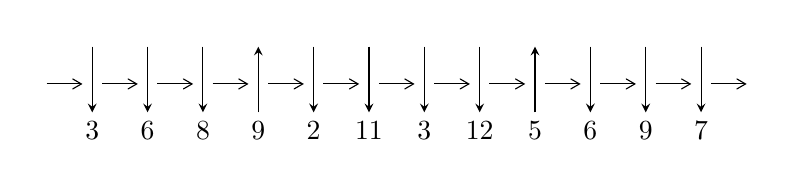
\begin{tikzpicture}[x=20pt, y=17pt]
	% nodes
	\node (C0) at (0, 0) {};
	\node (C1) at (1, 0) {};
	\node (C1U) at (1, +1) {};
	\node (C1D) at (1, -1) {3};

	\node (C2) at (2, 0) {};
	\node (C2U) at (2, +1) {};
	\node (C2D) at (2, -1) {6};

	\node (C3) at (3, 0) {};
	\node (C3U) at (3, +1) {};
	\node (C3D) at (3, -1) {8};

	\node (C4) at (4, 0) {};
	\node (C4U) at (4, +1) {};
	\node (C4D) at (4, -1) {9};

	\node (C5) at (5, 0) {};
	\node (C5U) at (5, +1) {};
	\node (C5D) at (5, -1) {2};

	\node (C6) at (6, 0) {};
	\node (C6U) at (6, +1) {};
	\node (C6D) at (6, -1) {11};

	\node (C7) at (7, 0) {};
	\node (C7U) at (7, +1) {};
	\node (C7D) at (7, -1) {3};

	\node (C8) at (8, 0) {};
	\node (C8U) at (8, +1) {};
	\node (C8D) at (8, -1) {12};

	\node (C9) at (9, 0) {};
	\node (C9U) at (9, +1) {};
	\node (C9D) at (9, -1) {5};

	\node (C10) at (10, 0) {};
	\node (C10U) at (10, +1) {};
	\node (C10D) at (10, -1) {6};

	\node (C11) at (11, 0) {};
	\node (C11U) at (11, +1) {};
	\node (C11D) at (11, -1) {9};

	\node (C12) at (12, 0) {};
	\node (C12U) at (12, +1) {};
	\node (C12D) at (12, -1) {7};
	\node (C13) at (13, 0) {};

	% arrows
	\draw[->,>={angle 60}]
	(C0) edge (C1) (C1) edge (C2) (C2) edge (C3) (C3) edge (C4) (C4) edge (C5) (C5) edge (C6) (C6) edge (C7) (C7) edge (C8) (C8) edge (C9) (C9) edge (C10) (C10) edge (C11) (C11) edge (C12) (C12) edge (C13) ;	\draw[->,>=stealth]
	(C1U) edge (C1D) (C2U) edge (C2D) (C3U) edge (C3D) (C4D) edge (C4U) (C5U) edge (C5D) (C6U) edge (C6D) (C7U) edge (C7D) (C8U) edge (C8D) (C9D) edge (C9U) (C10U) edge (C10D) (C11U) edge (C11D) (C12U) edge (C12D) ;
	\end{tikzpicture} \\
\hhline{~~} \\& 
\textbf{Solving Sequence} \\ \cline{2-2} 
 &
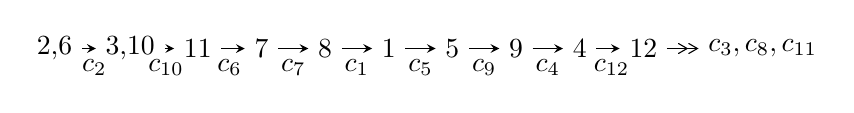
\begin{tikzpicture}[x=23pt, y=7pt]
	% node
	\node (A0) at (-1/8, 0) {2,6};
	\node (A1) at (17/16, 0) {3,10};
	\node (A2) at (17/8, 0) {11};
	\node (A3) at (25/8, 0) {7};
	\node (A4) at (33/8, 0) {8};
	\node (A5) at (41/8, 0) {1};
	\node (A6) at (49/8, 0) {5};
	\node (A7) at (57/8, 0) {9};
	\node (A8) at (65/8, 0) {4};
	\node (A9) at (73/8, 0) {12};
	\node (C1) at (1/2, -1) {$c_{2}$};
	\node (C2) at (13/8, -1) {$c_{10}$};
	\node (C3) at (21/8, -1) {$c_{6}$};
	\node (C4) at (29/8, -1) {$c_{7}$};
	\node (C5) at (37/8, -1) {$c_{1}$};
	\node (C6) at (45/8, -1) {$c_{5}$};
	\node (C7) at (53/8, -1) {$c_{9}$};
	\node (C8) at (61/8, -1) {$c_{4}$};
	\node (C9) at (69/8, -1) {$c_{12}$};
	\node (A10) at (11, 0) {$c_{3},c_{8},c_{11}$};

	% edge
	\draw[->,>=stealth]	
	(A0) edge (A1) (A1) edge (A2) (A2) edge (A3) (A3) edge (A4) (A4) edge (A5) (A5) edge (A6) (A6) edge (A7) (A7) edge (A8) (A8) edge (A9) ;
	\draw[->>,>={angle 60}]	
	(A9) edge (A10);
\end{tikzpicture} \\ 

\end{tabular} \\

\footnotetext{
The image of knot diagram is generated by the software ``\textbf{Draw programme}" developed by Andrew Bartholomew(\url{http://www.layer8.co.uk/maths/draw/index.htm\#Running-draw}), where we modified some parts for our purpose(\url{https://github.com/CATsTAILs/LinksPainter}).
}\phantom \\ \newline 
\centering \textbf{Ideals for irreducible components\footnotemark of $X_{\text{par}}$} 
 
\begin{align*}
I^u_{1}&=\langle 
339 u^{19}-3935 u^{18}+\cdots+809 b+2456,\;-1439 u^{19}+6826 u^{18}+\cdots+2427 a+13155,\\
\phantom{I^u_{1}}&\phantom{= \langle  }u^{20}-8 u^{19}+\cdots+12 u-3\rangle \\
I^u_{2}&=\langle 
- u^9 a-9 u^9+\cdots- a-15,\;-5 u^9 a- u^9+\cdots-7 a-3,\\
\phantom{I^u_{2}}&\phantom{= \langle  }u^{10}+2 u^9+u^8-3 u^7-2 u^6+2 u^5+3 u^4-2 u^3- u^2+2 u+1\rangle \\
I^u_{3}&=\langle 
2 u^{10}+9 u^9+14 u^8+u^7-24 u^6-23 u^5+11 u^4+29 u^3+7 u^2+b-13 u-5,\\
\phantom{I^u_{3}}&\phantom{= \langle  }-3 u^{10}-14 u^9-22 u^8+42 u^6+38 u^5-22 u^4-50 u^3-9 u^2+a+24 u+7,\\
\phantom{I^u_{3}}&\phantom{= \langle  }u^{11}+5 u^{10}+9 u^9+3 u^8-13 u^7-17 u^6+2 u^5+18 u^4+9 u^3-6 u^2-5 u-1\rangle \\
I^u_{4}&=\langle 
b^2+b-1,\;a+1,\;u-1\rangle \\
\\
I^v_{1}&=\langle 
a,\;b+1,\;v-1\rangle \\
\end{align*}
\raggedright * 5 irreducible components of $\dim_{\mathbb{C}}=0$, with total 54 representations.\\
\footnotetext{All coefficients of polynomials are rational numbers. But the coefficients are sometimes approximated in decimal forms when there is not enough margin.}
\newpage
\renewcommand{\arraystretch}{1}
\centering \section*{I. $I^u_{1}= \langle 339 u^{19}-3935 u^{18}+\cdots+809 b+2456,\;-1439 u^{19}+6826 u^{18}+\cdots+2427 a+13155,\;u^{20}-8 u^{19}+\cdots+12 u-3 \rangle$}
\flushleft \textbf{(i) Arc colorings}\\
\begin{tabular}{m{7pt} m{180pt} m{7pt} m{180pt} }
\flushright $a_{2}=$&$\begin{pmatrix}1\\0\end{pmatrix}$ \\
\flushright $a_{6}=$&$\begin{pmatrix}0\\u\end{pmatrix}$ \\
\flushright $a_{3}=$&$\begin{pmatrix}1\\u^2\end{pmatrix}$ \\
\flushright $a_{10}=$&$\begin{pmatrix}0.592913 u^{19}-2.81253 u^{18}+\cdots+12.5904 u-5.42027\\-0.419036 u^{19}+4.86403 u^{18}+\cdots+14.5278 u-3.03585\end{pmatrix}$ \\
\flushright $a_{11}=$&$\begin{pmatrix}0.592913 u^{19}-2.81253 u^{18}+\cdots+12.5904 u-5.42027\\1.53276 u^{19}-10.3375 u^{18}+\cdots-6.86279 u+2.75649\end{pmatrix}$ \\
\flushright $a_{7}=$&$\begin{pmatrix}-1.20231 u^{19}+7.31685 u^{18}+\cdots-4.78451 u+3.02596\\-1.03585 u^{19}+7.02967 u^{18}+\cdots+3.81211 u-0.846724\end{pmatrix}$ \\
\flushright $a_{8}=$&$\begin{pmatrix}-2.01937 u^{19}+15.3379 u^{18}+\cdots+15.4157 u-3.03214\\2.30161 u^{19}-16.5600 u^{18}+\cdots-16.4536 u+3.60692\end{pmatrix}$ \\
\flushright $a_{1}=$&$\begin{pmatrix}- u^2+1\\- u^4\end{pmatrix}$ \\
\flushright $a_{5}=$&$\begin{pmatrix}u\\u\end{pmatrix}$ \\
\flushright $a_{9}=$&$\begin{pmatrix}-0.918830 u^{19}+5.81788 u^{18}+\cdots+10.5979 u-4.16316\\-1.93078 u^{19}+13.4944 u^{18}+\cdots+12.5352 u-1.77874\end{pmatrix}$ \\
\flushright $a_{4}=$&$\begin{pmatrix}-0.952616 u^{19}+6.38607 u^{18}+\cdots+9.11042 u-2.28307\\0.817058 u^{19}-8.02101 u^{18}+\cdots-20.2002 u+6.05810\end{pmatrix}$ \\
\flushright $a_{12}=$&$\begin{pmatrix}0.753605 u^{19}-5.80758 u^{18}+\cdots-4.77421 u+2.27194\\-1.60939 u^{19}+12.5043 u^{18}+\cdots+19.8059 u-5.39431\end{pmatrix}$\\&\end{tabular}
\flushleft \textbf{(ii) Obstruction class $= -1$}\\~\\
\flushleft \textbf{(iii) Cusp Shapes $= -\frac{277}{809} u^{19}+\frac{4609}{809} u^{18}+\cdots+\frac{33642}{809} u-\frac{32682}{809}$}\\~\\
\newpage\renewcommand{\arraystretch}{1}
\flushleft \textbf{(iv) u-Polynomials at the component}\newline \\
\begin{tabular}{m{50pt}|m{274pt}}
Crossings & \hspace{64pt}u-Polynomials at each crossing \\
\hline $$\begin{aligned}c_{1}\end{aligned}$$&$\begin{aligned}
&u^{20}+8 u^{19}+\cdots+150 u+9
\end{aligned}$\\
\hline $$\begin{aligned}c_{2},c_{5}\end{aligned}$$&$\begin{aligned}
&u^{20}+8 u^{19}+\cdots-12 u-3
\end{aligned}$\\
\hline $$\begin{aligned}c_{3},c_{7}\end{aligned}$$&$\begin{aligned}
&u^{20}-2 u^{19}+\cdots+u+1
\end{aligned}$\\
\hline $$\begin{aligned}c_{4},c_{9}\end{aligned}$$&$\begin{aligned}
&u^{20}-8 u^{18}+\cdots+3 u+1
\end{aligned}$\\
\hline $$\begin{aligned}c_{6},c_{10}\end{aligned}$$&$\begin{aligned}
&u^{20}+6 u^{18}+\cdots+9 u+1
\end{aligned}$\\
\hline $$\begin{aligned}c_{8},c_{11}\end{aligned}$$&$\begin{aligned}
&u^{20}-7 u^{19}+\cdots+12 u-3
\end{aligned}$\\
\hline $$\begin{aligned}c_{12}\end{aligned}$$&$\begin{aligned}
&u^{20}+21 u^{19}+\cdots+6656 u+512
\end{aligned}$\\
\hline
\end{tabular}\\~\\
\newpage\renewcommand{\arraystretch}{1}
\flushleft \textbf{(v) Riley Polynomials at the component}\newline \\
\begin{tabular}{m{50pt}|m{274pt}}
Crossings & \hspace{64pt}Riley Polynomials at each crossing \\
\hline $$\begin{aligned}c_{1}\end{aligned}$$&$\begin{aligned}
&y^{20}+16 y^{19}+\cdots-5202 y+81
\end{aligned}$\\
\hline $$\begin{aligned}c_{2},c_{5}\end{aligned}$$&$\begin{aligned}
&y^{20}-8 y^{19}+\cdots-150 y+9
\end{aligned}$\\
\hline $$\begin{aligned}c_{3},c_{7}\end{aligned}$$&$\begin{aligned}
&y^{20}-28 y^{19}+\cdots+7 y+1
\end{aligned}$\\
\hline $$\begin{aligned}c_{4},c_{9}\end{aligned}$$&$\begin{aligned}
&y^{20}-16 y^{19}+\cdots+5 y+1
\end{aligned}$\\
\hline $$\begin{aligned}c_{6},c_{10}\end{aligned}$$&$\begin{aligned}
&y^{20}+12 y^{19}+\cdots-21 y+1
\end{aligned}$\\
\hline $$\begin{aligned}c_{8},c_{11}\end{aligned}$$&$\begin{aligned}
&y^{20}+11 y^{19}+\cdots-132 y+9
\end{aligned}$\\
\hline $$\begin{aligned}c_{12}\end{aligned}$$&$\begin{aligned}
&y^{20}-9 y^{19}+\cdots-2621440 y+262144
\end{aligned}$\\
\hline
\end{tabular}\\~\\
\newpage\flushleft \textbf{(vi) Complex Volumes and Cusp Shapes}
$$\begin{array}{c|c|c}  
\text{Solutions to }I^u_{1}& \I (\text{vol} + \sqrt{-1}CS) & \text{Cusp shape}\\
 \hline 
\begin{aligned}
u &= \phantom{-}0.739766 + 0.810627 I \\
a &= -0.332052 - 0.863055 I \\
b &= -1.178040 - 0.181845 I\end{aligned}
 & -1.201950 + 0.670281 I & -8.29063 + 0.06466 I \\ \hline\begin{aligned}
u &= \phantom{-}0.739766 - 0.810627 I \\
a &= -0.332052 + 0.863055 I \\
b &= -1.178040 + 0.181845 I\end{aligned}
 & -1.201950 - 0.670281 I & -8.29063 - 0.06466 I \\ \hline\begin{aligned}
u &= \phantom{-}0.579374 + 0.935372 I \\
a &= -1.121180 - 0.363583 I \\
b &= -0.996152 + 0.778841 I\end{aligned}
 & \phantom{-}6.00051 - 2.90762 I & -6.41870 + 3.35662 I \\ \hline\begin{aligned}
u &= \phantom{-}0.579374 - 0.935372 I \\
a &= -1.121180 + 0.363583 I \\
b &= -0.996152 - 0.778841 I\end{aligned}
 & \phantom{-}6.00051 + 2.90762 I & -6.41870 - 3.35662 I \\ \hline\begin{aligned}
u &= \phantom{-}0.725363\phantom{ +0.000000I} \\
a &= \phantom{-}0.248162\phantom{ +0.000000I} \\
b &= -0.655437\phantom{ +0.000000I}\end{aligned}
 & -1.32826\phantom{ +0.000000I} & -7.40410\phantom{ +0.000000I} \\ \hline\begin{aligned}
u &= -0.641694 + 0.281021 I \\
a &= \phantom{-}1.66993 - 0.14677 I \\
b &= \phantom{-}0.666818 - 0.229080 I\end{aligned}
 & \phantom{-}2.15316 + 3.41819 I & \phantom{-}1.21797 - 1.44999 I \\ \hline\begin{aligned}
u &= -0.641694 - 0.281021 I \\
a &= \phantom{-}1.66993 + 0.14677 I \\
b &= \phantom{-}0.666818 + 0.229080 I\end{aligned}
 & \phantom{-}2.15316 - 3.41819 I & \phantom{-}1.21797 + 1.44999 I \\ \hline\begin{aligned}
u &= \phantom{-}1.009590 + 0.838851 I \\
a &= \phantom{-}1.119650 + 0.309640 I \\
b &= \phantom{-}1.50399 - 1.02071 I\end{aligned}
 & -1.88231 - 6.91835 I & -9.67007 + 4.45150 I \\ \hline\begin{aligned}
u &= \phantom{-}1.009590 - 0.838851 I \\
a &= \phantom{-}1.119650 - 0.309640 I \\
b &= \phantom{-}1.50399 + 1.02071 I\end{aligned}
 & -1.88231 + 6.91835 I & -9.67007 - 4.45150 I \\ \hline\begin{aligned}
u &= \phantom{-}0.522186 + 0.274434 I \\
a &= \phantom{-}0.715817 + 0.493479 I \\
b &= \phantom{-}0.035362 - 0.930126 I\end{aligned}
 & -0.818282 - 1.020500 I & -8.50734 + 6.76581 I\\
 \hline 
 \end{array}$$\newpage$$\begin{array}{c|c|c}  
\text{Solutions to }I^u_{1}& \I (\text{vol} + \sqrt{-1}CS) & \text{Cusp shape}\\
 \hline 
\begin{aligned}
u &= \phantom{-}0.522186 - 0.274434 I \\
a &= \phantom{-}0.715817 - 0.493479 I \\
b &= \phantom{-}0.035362 + 0.930126 I\end{aligned}
 & -0.818282 + 1.020500 I & -8.50734 - 6.76581 I \\ \hline\begin{aligned}
u &= \phantom{-}0.82856 + 1.18903 I \\
a &= \phantom{-}0.665734 + 0.836247 I \\
b &= \phantom{-}1.275630 + 0.188413 I\end{aligned}
 & \phantom{-}1.33376 + 6.29384 I & -5.85142 - 3.79279 I \\ \hline\begin{aligned}
u &= \phantom{-}0.82856 - 1.18903 I \\
a &= \phantom{-}0.665734 - 0.836247 I \\
b &= \phantom{-}1.275630 - 0.188413 I\end{aligned}
 & \phantom{-}1.33376 - 6.29384 I & -5.85142 + 3.79279 I \\ \hline\begin{aligned}
u &= \phantom{-}1.28182 + 0.74255 I \\
a &= \phantom{-}0.465354 + 0.427519 I \\
b &= \phantom{-}1.176510 + 0.070724 I\end{aligned}
 & \phantom{-}3.78911 - 3.43912 I & -5.47667 + 2.61689 I \\ \hline\begin{aligned}
u &= \phantom{-}1.28182 - 0.74255 I \\
a &= \phantom{-}0.465354 - 0.427519 I \\
b &= \phantom{-}1.176510 - 0.070724 I\end{aligned}
 & \phantom{-}3.78911 + 3.43912 I & -5.47667 - 2.61689 I \\ \hline\begin{aligned}
u &= \phantom{-}1.14224 + 0.95656 I \\
a &= -1.149420 - 0.323355 I \\
b &= -1.65497 + 0.80309 I\end{aligned}
 & \phantom{-}0.28633 - 13.95250 I & -7.83055 + 7.44247 I \\ \hline\begin{aligned}
u &= \phantom{-}1.14224 - 0.95656 I \\
a &= -1.149420 + 0.323355 I \\
b &= -1.65497 - 0.80309 I\end{aligned}
 & \phantom{-}0.28633 + 13.95250 I & -7.83055 - 7.44247 I \\ \hline\begin{aligned}
u &= -1.65206 + 0.05162 I \\
a &= -0.199755 - 0.409902 I \\
b &= -0.127470 - 0.253935 I\end{aligned}
 & -9.08165 + 2.30266 I & -5.04461 + 4.85763 I \\ \hline\begin{aligned}
u &= -1.65206 - 0.05162 I \\
a &= -0.199755 + 0.409902 I \\
b &= -0.127470 + 0.253935 I\end{aligned}
 & -9.08165 - 2.30266 I & -5.04461 - 4.85763 I \\ \hline\begin{aligned}
u &= -0.344930\phantom{ +0.000000I} \\
a &= -2.91630\phantom{ +0.000000I} \\
b &= -0.747935\phantom{ +0.000000I}\end{aligned}
 & -1.47402\phantom{ +0.000000I} & -6.85190\phantom{ +0.000000I}\\
 \hline 
 \end{array}$$\newpage\newpage\renewcommand{\arraystretch}{1}
\centering \section*{II. $I^u_{2}= \langle - u^9 a-9 u^9+\cdots- a-15,\;-5 u^9 a- u^9+\cdots-7 a-3,\;u^{10}+2 u^9+\cdots+2 u+1 \rangle$}
\flushleft \textbf{(i) Arc colorings}\\
\begin{tabular}{m{7pt} m{180pt} m{7pt} m{180pt} }
\flushright $a_{2}=$&$\begin{pmatrix}1\\0\end{pmatrix}$ \\
\flushright $a_{6}=$&$\begin{pmatrix}0\\u\end{pmatrix}$ \\
\flushright $a_{3}=$&$\begin{pmatrix}1\\u^2\end{pmatrix}$ \\
\flushright $a_{10}=$&$\begin{pmatrix}a\\\frac{1}{2} u^9 a+\frac{9}{2} u^9+\cdots+\frac{1}{2} a+\frac{15}{2}\end{pmatrix}$ \\
\flushright $a_{11}=$&$\begin{pmatrix}a\\\frac{1}{2} u^9 a+\frac{9}{2} u^9+\cdots+\frac{1}{2} a+\frac{15}{2}\end{pmatrix}$ \\
\flushright $a_{7}=$&$\begin{pmatrix}3 u^9 a+u^9+\cdots+5 a+1\\-\frac{1}{2} u^9 a+\frac{1}{2} u^9+\cdots-\frac{1}{2} a-\frac{1}{2}\end{pmatrix}$ \\
\flushright $a_{8}=$&$\begin{pmatrix}\frac{9}{2} u^9 a+\frac{1}{2} u^9+\cdots+\frac{15}{2} a+\frac{3}{2}\\-1\end{pmatrix}$ \\
\flushright $a_{1}=$&$\begin{pmatrix}- u^2+1\\- u^4\end{pmatrix}$ \\
\flushright $a_{5}=$&$\begin{pmatrix}u\\u\end{pmatrix}$ \\
\flushright $a_{9}=$&$\begin{pmatrix}-\frac{1}{2} u^9 a-\frac{3}{2} u^9+\cdots+\frac{1}{2} a-\frac{5}{2}\\3 u^9+4 u^8-9 u^6+u^5+7 u^4+4 u^3+a u-10 u^2+3 u+5\end{pmatrix}$ \\
\flushright $a_{4}=$&$\begin{pmatrix}6 u^9 a+u^9+\cdots+10 a+2\\\frac{3}{2} u^9 a-\frac{1}{2} u^9+\cdots+\frac{5}{2} a+\frac{1}{2}\end{pmatrix}$ \\
\flushright $a_{12}=$&$\begin{pmatrix}3 u^9 a+u^9+\cdots+5 a+2\\-\frac{1}{2} u^9 a+\frac{1}{2} u^9+\cdots-\frac{1}{2} a-\frac{1}{2}\end{pmatrix}$\\&\end{tabular}
\flushleft \textbf{(ii) Obstruction class $= -1$}\\~\\
\flushleft \textbf{(iii) Cusp Shapes $= -11 u^9-17 u^8+37 u^6+3 u^5-35 u^4-20 u^3+38 u^2-3 u-35$}\\~\\
\newpage\renewcommand{\arraystretch}{1}
\flushleft \textbf{(iv) u-Polynomials at the component}\newline \\
\begin{tabular}{m{50pt}|m{274pt}}
Crossings & \hspace{64pt}u-Polynomials at each crossing \\
\hline $$\begin{aligned}c_{1}\end{aligned}$$&$\begin{aligned}
&(u^{10}+2 u^9+9 u^8+15 u^7+28 u^6+36 u^5+35 u^4+22 u^3+15 u^2+6 u+1)^{2}
\end{aligned}$\\
\hline $$\begin{aligned}c_{2},c_{5}\end{aligned}$$&$\begin{aligned}
&(u^{10}-2 u^9+u^8+3 u^7-2 u^6-2 u^5+3 u^4+2 u^3- u^2-2 u+1)^2
\end{aligned}$\\
\hline $$\begin{aligned}c_{3},c_{7}\end{aligned}$$&$\begin{aligned}
&u^{20}+2 u^{19}+\cdots-19 u+61
\end{aligned}$\\
\hline $$\begin{aligned}c_{4},c_{9}\end{aligned}$$&$\begin{aligned}
&u^{20}-6 u^{18}+\cdots-15 u+85
\end{aligned}$\\
\hline $$\begin{aligned}c_{6},c_{10}\end{aligned}$$&$\begin{aligned}
&u^{20}-3 u^{19}+\cdots-108 u+59
\end{aligned}$\\
\hline $$\begin{aligned}c_{8},c_{11}\end{aligned}$$&$\begin{aligned}
&(u^{10}+3 u^9+6 u^8+7 u^7+9 u^6+9 u^5+10 u^4+6 u^3+5 u^2+3 u+2)^2
\end{aligned}$\\
\hline $$\begin{aligned}c_{12}\end{aligned}$$&$\begin{aligned}
&(u-1)^{20}
\end{aligned}$\\
\hline
\end{tabular}\\~\\
\newpage\renewcommand{\arraystretch}{1}
\flushleft \textbf{(v) Riley Polynomials at the component}\newline \\
\begin{tabular}{m{50pt}|m{274pt}}
Crossings & \hspace{64pt}Riley Polynomials at each crossing \\
\hline $$\begin{aligned}c_{1}\end{aligned}$$&$\begin{aligned}
&(y^{10}+14 y^9+\cdots-6 y+1)^{2}
\end{aligned}$\\
\hline $$\begin{aligned}c_{2},c_{5}\end{aligned}$$&$\begin{aligned}
&(y^{10}-2 y^9+9 y^8-15 y^7+28 y^6-36 y^5+35 y^4-22 y^3+15 y^2-6 y+1)^{2}
\end{aligned}$\\
\hline $$\begin{aligned}c_{3},c_{7}\end{aligned}$$&$\begin{aligned}
&y^{20}-12 y^{19}+\cdots-40987 y+3721
\end{aligned}$\\
\hline $$\begin{aligned}c_{4},c_{9}\end{aligned}$$&$\begin{aligned}
&y^{20}-12 y^{19}+\cdots-97975 y+7225
\end{aligned}$\\
\hline $$\begin{aligned}c_{6},c_{10}\end{aligned}$$&$\begin{aligned}
&y^{20}+13 y^{19}+\cdots+76246 y+3481
\end{aligned}$\\
\hline $$\begin{aligned}c_{8},c_{11}\end{aligned}$$&$\begin{aligned}
&(y^{10}+3 y^9+\cdots+11 y+4)^{2}
\end{aligned}$\\
\hline $$\begin{aligned}c_{12}\end{aligned}$$&$\begin{aligned}
&(y-1)^{20}
\end{aligned}$\\
\hline
\end{tabular}\\~\\
\newpage\flushleft \textbf{(vi) Complex Volumes and Cusp Shapes}
$$\begin{array}{c|c|c}  
\text{Solutions to }I^u_{2}& \I (\text{vol} + \sqrt{-1}CS) & \text{Cusp shape}\\
 \hline 
\begin{aligned}
u &= \phantom{-}0.975430 + 0.320615 I \\
a &= -1.065150 + 0.247050 I \\
b &= -1.63832 + 0.24814 I\end{aligned}
 & -3.87176 + 0.60085 I & -13.31849 - 3.40041 I \\ \hline\begin{aligned}
u &= \phantom{-}0.975430 + 0.320615 I \\
a &= \phantom{-}0.880921 - 0.910530 I \\
b &= -0.559442 - 0.182706 I\end{aligned}
 & -3.87176 + 0.60085 I & -13.31849 - 3.40041 I \\ \hline\begin{aligned}
u &= \phantom{-}0.975430 - 0.320615 I \\
a &= -1.065150 - 0.247050 I \\
b &= -1.63832 - 0.24814 I\end{aligned}
 & -3.87176 - 0.60085 I & -13.31849 + 3.40041 I \\ \hline\begin{aligned}
u &= \phantom{-}0.975430 - 0.320615 I \\
a &= \phantom{-}0.880921 + 0.910530 I \\
b &= -0.559442 + 0.182706 I\end{aligned}
 & -3.87176 - 0.60085 I & -13.31849 + 3.40041 I \\ \hline\begin{aligned}
u &= \phantom{-}0.541733 + 0.670646 I \\
a &= \phantom{-}1.294850 - 0.350726 I \\
b &= \phantom{-}1.70668 - 0.48449 I\end{aligned}
 & -2.20007 - 4.58635 I & -7.79322 + 7.42430 I \\ \hline\begin{aligned}
u &= \phantom{-}0.541733 + 0.670646 I \\
a &= -0.49398 + 2.09684 I \\
b &= \phantom{-}0.312809 + 0.203725 I\end{aligned}
 & -2.20007 - 4.58635 I & -7.79322 + 7.42430 I \\ \hline\begin{aligned}
u &= \phantom{-}0.541733 - 0.670646 I \\
a &= \phantom{-}1.294850 + 0.350726 I \\
b &= \phantom{-}1.70668 + 0.48449 I\end{aligned}
 & -2.20007 + 4.58635 I & -7.79322 - 7.42430 I \\ \hline\begin{aligned}
u &= \phantom{-}0.541733 - 0.670646 I \\
a &= -0.49398 - 2.09684 I \\
b &= \phantom{-}0.312809 - 0.203725 I\end{aligned}
 & -2.20007 + 4.58635 I & -7.79322 - 7.42430 I \\ \hline\begin{aligned}
u &= -0.876556 + 1.026090 I \\
a &= -0.533352 + 0.614318 I \\
b &= -1.129040 - 0.385187 I\end{aligned}
 & \phantom{-}6.17677 + 1.75340 I & -6.60526 + 0.85033 I \\ \hline\begin{aligned}
u &= -0.876556 + 1.026090 I \\
a &= \phantom{-}1.221340 - 0.556605 I \\
b &= \phantom{-}1.54773 + 0.26490 I\end{aligned}
 & \phantom{-}6.17677 + 1.75340 I & -6.60526 + 0.85033 I\\
 \hline 
 \end{array}$$\newpage$$\begin{array}{c|c|c}  
\text{Solutions to }I^u_{2}& \I (\text{vol} + \sqrt{-1}CS) & \text{Cusp shape}\\
 \hline 
\begin{aligned}
u &= -0.876556 - 1.026090 I \\
a &= -0.533352 - 0.614318 I \\
b &= -1.129040 + 0.385187 I\end{aligned}
 & \phantom{-}6.17677 - 1.75340 I & -6.60526 - 0.85033 I \\ \hline\begin{aligned}
u &= -0.876556 - 1.026090 I \\
a &= \phantom{-}1.221340 + 0.556605 I \\
b &= \phantom{-}1.54773 - 0.26490 I\end{aligned}
 & \phantom{-}6.17677 - 1.75340 I & -6.60526 - 0.85033 I \\ \hline\begin{aligned}
u &= -0.580680 + 0.133301 I \\
a &= -0.062064 + 0.507460 I \\
b &= \phantom{-}0.18768 + 2.50740 I\end{aligned}
 & -4.85763 + 3.93250 I & -20.2791 - 6.7139 I \\ \hline\begin{aligned}
u &= -0.580680 + 0.133301 I \\
a &= -1.04621 + 3.04432 I \\
b &= -0.411614 - 1.128030 I\end{aligned}
 & -4.85763 + 3.93250 I & -20.2791 - 6.7139 I \\ \hline\begin{aligned}
u &= -0.580680 - 0.133301 I \\
a &= -0.062064 - 0.507460 I \\
b &= \phantom{-}0.18768 - 2.50740 I\end{aligned}
 & -4.85763 - 3.93250 I & -20.2791 + 6.7139 I \\ \hline\begin{aligned}
u &= -0.580680 - 0.133301 I \\
a &= -1.04621 - 3.04432 I \\
b &= -0.411614 + 1.128030 I\end{aligned}
 & -4.85763 - 3.93250 I & -20.2791 + 6.7139 I \\ \hline\begin{aligned}
u &= -1.059930 + 0.922349 I \\
a &= \phantom{-}0.797570 - 0.248575 I \\
b &= \phantom{-}1.51824 + 0.58719 I\end{aligned}
 & \phantom{-}5.57516 + 5.36397 I & -8.50388 - 6.50559 I \\ \hline\begin{aligned}
u &= -1.059930 + 0.922349 I \\
a &= -0.993922 + 0.803452 I \\
b &= -1.53472 - 0.22114 I\end{aligned}
 & \phantom{-}5.57516 + 5.36397 I & -8.50388 - 6.50559 I \\ \hline\begin{aligned}
u &= -1.059930 - 0.922349 I \\
a &= \phantom{-}0.797570 + 0.248575 I \\
b &= \phantom{-}1.51824 - 0.58719 I\end{aligned}
 & \phantom{-}5.57516 - 5.36397 I & -8.50388 + 6.50559 I \\ \hline\begin{aligned}
u &= -1.059930 - 0.922349 I \\
a &= -0.993922 - 0.803452 I \\
b &= -1.53472 + 0.22114 I\end{aligned}
 & \phantom{-}5.57516 - 5.36397 I & -8.50388 + 6.50559 I\\
 \hline 
 \end{array}$$\newpage\newpage\renewcommand{\arraystretch}{1}
\centering \section*{III. $I^u_{3}= \langle 2 u^{10}+9 u^9+\cdots+b-5,\;-3 u^{10}-14 u^9+\cdots+a+7,\;u^{11}+5 u^{10}+\cdots-5 u-1 \rangle$}
\flushleft \textbf{(i) Arc colorings}\\
\begin{tabular}{m{7pt} m{180pt} m{7pt} m{180pt} }
\flushright $a_{2}=$&$\begin{pmatrix}1\\0\end{pmatrix}$ \\
\flushright $a_{6}=$&$\begin{pmatrix}0\\u\end{pmatrix}$ \\
\flushright $a_{3}=$&$\begin{pmatrix}1\\u^2\end{pmatrix}$ \\
\flushright $a_{10}=$&$\begin{pmatrix}3 u^{10}+14 u^9+22 u^8-42 u^6-38 u^5+22 u^4+50 u^3+9 u^2-24 u-7\\-2 u^{10}-9 u^9+\cdots+13 u+5\end{pmatrix}$ \\
\flushright $a_{11}=$&$\begin{pmatrix}3 u^{10}+14 u^9+22 u^8-42 u^6-38 u^5+22 u^4+50 u^3+9 u^2-24 u-7\\-2 u^{10}-9 u^9+\cdots+11 u+4\end{pmatrix}$ \\
\flushright $a_{7}=$&$\begin{pmatrix}u^{10}+5 u^9+9 u^8+3 u^7-13 u^6-17 u^5+2 u^4+18 u^3+9 u^2-7 u-6\\u^{10}+4 u^9+5 u^8-2 u^7-11 u^6-6 u^5+8 u^4+9 u^3-2 u^2-4 u\end{pmatrix}$ \\
\flushright $a_{8}=$&$\begin{pmatrix}u^9+4 u^8+5 u^7-2 u^6-11 u^5-6 u^4+8 u^3+10 u^2-2 u-6\\- u^3- u^2+1\end{pmatrix}$ \\
\flushright $a_{1}=$&$\begin{pmatrix}- u^2+1\\- u^4\end{pmatrix}$ \\
\flushright $a_{5}=$&$\begin{pmatrix}u\\u\end{pmatrix}$ \\
\flushright $a_{9}=$&$\begin{pmatrix}4 u^{10}+18 u^9+\cdots-29 u-9\\- u^{10}-5 u^9-9 u^8-3 u^7+13 u^6+16 u^5-4 u^4-18 u^3-6 u^2+8 u+3\end{pmatrix}$ \\
\flushright $a_{4}=$&$\begin{pmatrix}- u^{10}-4 u^9-4 u^8+5 u^7+13 u^6+2 u^5-15 u^4-9 u^3+8 u^2+8 u-4\\u^{10}+4 u^9+5 u^8-2 u^7-11 u^6-6 u^5+8 u^4+10 u^3- u^2-5 u\end{pmatrix}$ \\
\flushright $a_{12}=$&$\begin{pmatrix}- u^{10}-5 u^9-9 u^8-3 u^7+13 u^6+17 u^5-3 u^4-20 u^3-10 u^2+8 u+7\\- u^{10}-4 u^9-5 u^8+2 u^7+10 u^6+4 u^5-9 u^4-8 u^3+3 u^2+4 u\end{pmatrix}$\\&\end{tabular}
\flushleft \textbf{(ii) Obstruction class $= 1$}\\~\\
\flushleft \textbf{(iii) Cusp Shapes $= u^{10}+6 u^9+10 u^8- u^7-24 u^6-21 u^5+17 u^4+35 u^3+5 u^2-26 u-14$}\\~\\
\newpage\renewcommand{\arraystretch}{1}
\flushleft \textbf{(iv) u-Polynomials at the component}\newline \\
\begin{tabular}{m{50pt}|m{274pt}}
Crossings & \hspace{64pt}u-Polynomials at each crossing \\
\hline $$\begin{aligned}c_{1}\end{aligned}$$&$\begin{aligned}
&u^{11}-7 u^{10}+\cdots+13 u-1
\end{aligned}$\\
\hline $$\begin{aligned}c_{2}\end{aligned}$$&$\begin{aligned}
&u^{11}+5 u^{10}+\cdots-5 u-1
\end{aligned}$\\
\hline $$\begin{aligned}c_{3}\end{aligned}$$&$\begin{aligned}
&u^{11}- u^{10}+\cdots+6 u-1
\end{aligned}$\\
\hline $$\begin{aligned}c_{4}\end{aligned}$$&$\begin{aligned}
&u^{11}+u^{10}- u^9-2 u^8-5 u^7+4 u^6+12 u^5-4 u^4+u^3+5 u^2-1
\end{aligned}$\\
\hline $$\begin{aligned}c_{5}\end{aligned}$$&$\begin{aligned}
&u^{11}-5 u^{10}+\cdots-5 u+1
\end{aligned}$\\
\hline $$\begin{aligned}c_{6}\end{aligned}$$&$\begin{aligned}
&u^{11}+u^{10}+5 u^9+5 u^8+9 u^7+8 u^6+6 u^5- u^3-6 u^2-2 u-1
\end{aligned}$\\
\hline $$\begin{aligned}c_{7}\end{aligned}$$&$\begin{aligned}
&u^{11}+u^{10}+\cdots+6 u+1
\end{aligned}$\\
\hline $$\begin{aligned}c_{8}\end{aligned}$$&$\begin{aligned}
&u^{11}-4 u^{10}+\cdots+15 u-5
\end{aligned}$\\
\hline $$\begin{aligned}c_{9}\end{aligned}$$&$\begin{aligned}
&u^{11}- u^{10}- u^9+2 u^8-5 u^7-4 u^6+12 u^5+4 u^4+u^3-5 u^2+1
\end{aligned}$\\
\hline $$\begin{aligned}c_{10}\end{aligned}$$&$\begin{aligned}
&u^{11}- u^{10}+5 u^9-5 u^8+9 u^7-8 u^6+6 u^5- u^3+6 u^2-2 u+1
\end{aligned}$\\
\hline $$\begin{aligned}c_{11}\end{aligned}$$&$\begin{aligned}
&u^{11}+4 u^{10}+\cdots+15 u+5
\end{aligned}$\\
\hline $$\begin{aligned}c_{12}\end{aligned}$$&$\begin{aligned}
&u^{11}-3 u^{10}- u^8+8 u^7+8 u^6+10 u^5-13 u^4-17 u^3-8 u^2+11 u+5
\end{aligned}$\\
\hline
\end{tabular}\\~\\
\newpage\renewcommand{\arraystretch}{1}
\flushleft \textbf{(v) Riley Polynomials at the component}\newline \\
\begin{tabular}{m{50pt}|m{274pt}}
Crossings & \hspace{64pt}Riley Polynomials at each crossing \\
\hline $$\begin{aligned}c_{1}\end{aligned}$$&$\begin{aligned}
&y^{11}+y^{10}+\cdots-11 y-1
\end{aligned}$\\
\hline $$\begin{aligned}c_{2},c_{5}\end{aligned}$$&$\begin{aligned}
&y^{11}-7 y^{10}+\cdots+13 y-1
\end{aligned}$\\
\hline $$\begin{aligned}c_{3},c_{7}\end{aligned}$$&$\begin{aligned}
&y^{11}-7 y^{10}+\cdots+8 y-1
\end{aligned}$\\
\hline $$\begin{aligned}c_{4},c_{9}\end{aligned}$$&$\begin{aligned}
&y^{11}-3 y^{10}+\cdots+10 y-1
\end{aligned}$\\
\hline $$\begin{aligned}c_{6},c_{10}\end{aligned}$$&$\begin{aligned}
&y^{11}+9 y^{10}+\cdots-8 y-1
\end{aligned}$\\
\hline $$\begin{aligned}c_{8},c_{11}\end{aligned}$$&$\begin{aligned}
&y^{11}+8 y^{10}+\cdots-65 y-25
\end{aligned}$\\
\hline $$\begin{aligned}c_{12}\end{aligned}$$&$\begin{aligned}
&y^{11}-9 y^{10}+\cdots+201 y-25
\end{aligned}$\\
\hline
\end{tabular}\\~\\
\newpage\flushleft \textbf{(vi) Complex Volumes and Cusp Shapes}
$$\begin{array}{c|c|c}  
\text{Solutions to }I^u_{3}& \I (\text{vol} + \sqrt{-1}CS) & \text{Cusp shape}\\
 \hline 
\begin{aligned}
u &= \phantom{-}0.888248 + 0.348807 I \\
a &= \phantom{-}1.094700 + 0.166339 I \\
b &= \phantom{-}0.518352 + 0.184714 I\end{aligned}
 & \phantom{-}1.62880 - 3.55605 I & -13.8351 + 4.8849 I \\ \hline\begin{aligned}
u &= \phantom{-}0.888248 - 0.348807 I \\
a &= \phantom{-}1.094700 - 0.166339 I \\
b &= \phantom{-}0.518352 - 0.184714 I\end{aligned}
 & \phantom{-}1.62880 + 3.55605 I & -13.8351 - 4.8849 I \\ \hline\begin{aligned}
u &= \phantom{-}0.865988\phantom{ +0.000000I} \\
a &= -0.906257\phantom{ +0.000000I} \\
b &= -0.420586\phantom{ +0.000000I}\end{aligned}
 & -2.51061\phantom{ +0.000000I} & -16.1470\phantom{ +0.000000I} \\ \hline\begin{aligned}
u &= -0.794068 + 1.051540 I \\
a &= -1.013640 + 0.571990 I \\
b &= -1.35569 - 0.45895 I\end{aligned}
 & \phantom{-}7.94404 + 2.78344 I & -1.36367 - 2.55365 I \\ \hline\begin{aligned}
u &= -0.794068 - 1.051540 I \\
a &= -1.013640 - 0.571990 I \\
b &= -1.35569 + 0.45895 I\end{aligned}
 & \phantom{-}7.94404 - 2.78344 I & -1.36367 + 2.55365 I \\ \hline\begin{aligned}
u &= -1.12350 + 0.92492 I \\
a &= \phantom{-}0.823218 - 0.546732 I \\
b &= \phantom{-}1.52074 + 0.25018 I\end{aligned}
 & \phantom{-}6.92380 + 4.41989 I & -2.52937 - 2.98344 I \\ \hline\begin{aligned}
u &= -1.12350 - 0.92492 I \\
a &= \phantom{-}0.823218 + 0.546732 I \\
b &= \phantom{-}1.52074 - 0.25018 I\end{aligned}
 & \phantom{-}6.92380 - 4.41989 I & -2.52937 + 2.98344 I \\ \hline\begin{aligned}
u &= -1.56100 + 0.06449 I \\
a &= -0.120564 + 0.249710 I \\
b &= -0.383171 + 0.664642 I\end{aligned}
 & -9.38029 - 2.74226 I & -13.9541 + 7.1206 I \\ \hline\begin{aligned}
u &= -1.56100 - 0.06449 I \\
a &= -0.120564 - 0.249710 I \\
b &= -0.383171 - 0.664642 I\end{aligned}
 & -9.38029 + 2.74226 I & -13.9541 - 7.1206 I \\ \hline\begin{aligned}
u &= -0.342676 + 0.154468 I \\
a &= \phantom{-}1.16941 - 2.73498 I \\
b &= \phantom{-}0.41006 + 1.60424 I\end{aligned}
 & -4.21611 + 3.79963 I & -5.24446 - 3.20279 I\\
 \hline 
 \end{array}$$\newpage$$\begin{array}{c|c|c}  
\text{Solutions to }I^u_{3}& \I (\text{vol} + \sqrt{-1}CS) & \text{Cusp shape}\\
 \hline 
\begin{aligned}
u &= -0.342676 - 0.154468 I \\
a &= \phantom{-}1.16941 + 2.73498 I \\
b &= \phantom{-}0.41006 - 1.60424 I\end{aligned}
 & -4.21611 - 3.79963 I & -5.24446 + 3.20279 I\\
 \hline 
 \end{array}$$\newpage\newpage\renewcommand{\arraystretch}{1}
\centering \section*{IV. $I^u_{4}= \langle b^2+b-1,\;a+1,\;u-1 \rangle$}
\flushleft \textbf{(i) Arc colorings}\\
\begin{tabular}{m{7pt} m{180pt} m{7pt} m{180pt} }
\flushright $a_{2}=$&$\begin{pmatrix}1\\0\end{pmatrix}$ \\
\flushright $a_{6}=$&$\begin{pmatrix}0\\1\end{pmatrix}$ \\
\flushright $a_{3}=$&$\begin{pmatrix}1\\1\end{pmatrix}$ \\
\flushright $a_{10}=$&$\begin{pmatrix}-1\\b\end{pmatrix}$ \\
\flushright $a_{11}=$&$\begin{pmatrix}-1\\b-1\end{pmatrix}$ \\
\flushright $a_{7}=$&$\begin{pmatrix}-1\\b\end{pmatrix}$ \\
\flushright $a_{8}=$&$\begin{pmatrix}- b-2\\-1\end{pmatrix}$ \\
\flushright $a_{1}=$&$\begin{pmatrix}0\\-1\end{pmatrix}$ \\
\flushright $a_{5}=$&$\begin{pmatrix}1\\1\end{pmatrix}$ \\
\flushright $a_{9}=$&$\begin{pmatrix}- b-2\\-1\end{pmatrix}$ \\
\flushright $a_{4}=$&$\begin{pmatrix}-2 b-2\\- b\end{pmatrix}$ \\
\flushright $a_{12}=$&$\begin{pmatrix}-1\\b-1\end{pmatrix}$\\&\end{tabular}
\flushleft \textbf{(ii) Obstruction class $= 1$}\\~\\
\flushleft \textbf{(iii) Cusp Shapes $= -7$}\\~\\
\newpage\renewcommand{\arraystretch}{1}
\flushleft \textbf{(iv) u-Polynomials at the component}\newline \\
\begin{tabular}{m{50pt}|m{274pt}}
Crossings & \hspace{64pt}u-Polynomials at each crossing \\
\hline $$\begin{aligned}c_{1},c_{2},c_{6}\end{aligned}$$&$\begin{aligned}
&(u-1)^2
\end{aligned}$\\
\hline $$\begin{aligned}c_{3},c_{4}\end{aligned}$$&$\begin{aligned}
&u^2- u-1
\end{aligned}$\\
\hline $$\begin{aligned}c_{5},c_{10},c_{12}\end{aligned}$$&$\begin{aligned}
&(u+1)^2
\end{aligned}$\\
\hline $$\begin{aligned}c_{7},c_{9}\end{aligned}$$&$\begin{aligned}
&u^2+u-1
\end{aligned}$\\
\hline $$\begin{aligned}c_{8},c_{11}\end{aligned}$$&$\begin{aligned}
&u^2
\end{aligned}$\\
\hline
\end{tabular}\\~\\
\newpage\renewcommand{\arraystretch}{1}
\flushleft \textbf{(v) Riley Polynomials at the component}\newline \\
\begin{tabular}{m{50pt}|m{274pt}}
Crossings & \hspace{64pt}Riley Polynomials at each crossing \\
\hline $$\begin{aligned}c_{1},c_{2},c_{5}\\c_{6},c_{10},c_{12}\end{aligned}$$&$\begin{aligned}
&(y-1)^2
\end{aligned}$\\
\hline $$\begin{aligned}c_{3},c_{4},c_{7}\\c_{9}\end{aligned}$$&$\begin{aligned}
&y^2-3 y+1
\end{aligned}$\\
\hline $$\begin{aligned}c_{8},c_{11}\end{aligned}$$&$\begin{aligned}
&y^2
\end{aligned}$\\
\hline
\end{tabular}\\~\\
\newpage\flushleft \textbf{(vi) Complex Volumes and Cusp Shapes}
$$\begin{array}{c|c|c}  
\text{Solutions to }I^u_{4}& \I (\text{vol} + \sqrt{-1}CS) & \text{Cusp shape}\\
 \hline 
\begin{aligned}
u &= \phantom{-}1.00000\phantom{ +0.000000I} \\
a &= -1.00000\phantom{ +0.000000I} \\
b &= \phantom{-}0.618034\phantom{ +0.000000I}\end{aligned}
 & -3.28987\phantom{ +0.000000I} & -7.00000\phantom{ +0.000000I} \\ \hline\begin{aligned}
u &= \phantom{-}1.00000\phantom{ +0.000000I} \\
a &= -1.00000\phantom{ +0.000000I} \\
b &= -1.61803\phantom{ +0.000000I}\end{aligned}
 & -3.28987\phantom{ +0.000000I} & -7.00000\phantom{ +0.000000I}\\
 \hline 
 \end{array}$$\newpage\newpage\renewcommand{\arraystretch}{1}
\centering \section*{V. $I^v_{1}= \langle a,\;b+1,\;v-1 \rangle$}
\flushleft \textbf{(i) Arc colorings}\\
\begin{tabular}{m{7pt} m{180pt} m{7pt} m{180pt} }
\flushright $a_{2}=$&$\begin{pmatrix}1\\0\end{pmatrix}$ \\
\flushright $a_{6}=$&$\begin{pmatrix}1\\0\end{pmatrix}$ \\
\flushright $a_{3}=$&$\begin{pmatrix}1\\0\end{pmatrix}$ \\
\flushright $a_{10}=$&$\begin{pmatrix}0\\-1\end{pmatrix}$ \\
\flushright $a_{11}=$&$\begin{pmatrix}1\\-1\end{pmatrix}$ \\
\flushright $a_{7}=$&$\begin{pmatrix}0\\1\end{pmatrix}$ \\
\flushright $a_{8}=$&$\begin{pmatrix}-1\\1\end{pmatrix}$ \\
\flushright $a_{1}=$&$\begin{pmatrix}1\\0\end{pmatrix}$ \\
\flushright $a_{5}=$&$\begin{pmatrix}1\\0\end{pmatrix}$ \\
\flushright $a_{9}=$&$\begin{pmatrix}1\\-1\end{pmatrix}$ \\
\flushright $a_{4}=$&$\begin{pmatrix}0\\1\end{pmatrix}$ \\
\flushright $a_{12}=$&$\begin{pmatrix}1\\-1\end{pmatrix}$\\&\end{tabular}
\flushleft \textbf{(ii) Obstruction class $= -1$}\\~\\
\flushleft \textbf{(iii) Cusp Shapes $= -6$}\\~\\
\newpage\renewcommand{\arraystretch}{1}
\flushleft \textbf{(iv) u-Polynomials at the component}\newline \\
\begin{tabular}{m{50pt}|m{274pt}}
Crossings & \hspace{64pt}u-Polynomials at each crossing \\
\hline $$\begin{aligned}c_{1},c_{2},c_{5}\\c_{8},c_{11}\end{aligned}$$&$\begin{aligned}
&u
\end{aligned}$\\
\hline $$\begin{aligned}c_{3},c_{4},c_{6}\\c_{7},c_{9},c_{10}\\c_{12}\end{aligned}$$&$\begin{aligned}
&u+1
\end{aligned}$\\
\hline
\end{tabular}\\~\\
\newpage\renewcommand{\arraystretch}{1}
\flushleft \textbf{(v) Riley Polynomials at the component}\newline \\
\begin{tabular}{m{50pt}|m{274pt}}
Crossings & \hspace{64pt}Riley Polynomials at each crossing \\
\hline $$\begin{aligned}c_{1},c_{2},c_{5}\\c_{8},c_{11}\end{aligned}$$&$\begin{aligned}
&y
\end{aligned}$\\
\hline $$\begin{aligned}c_{3},c_{4},c_{6}\\c_{7},c_{9},c_{10}\\c_{12}\end{aligned}$$&$\begin{aligned}
&y-1
\end{aligned}$\\
\hline
\end{tabular}\\~\\
\newpage\flushleft \textbf{(vi) Complex Volumes and Cusp Shapes}
$$\begin{array}{c|c|c}  
\text{Solutions to }I^v_{1}& \I (\text{vol} + \sqrt{-1}CS) & \text{Cusp shape}\\
 \hline 
\begin{aligned}
v &= \phantom{-}1.00000\phantom{ +0.000000I} \\
a &= \phantom{-0.000000 } 0 \\
b &= -1.00000\phantom{ +0.000000I}\end{aligned}
 & -1.64493\phantom{ +0.000000I} & -6.00000\phantom{ +0.000000I}\\
 \hline 
 \end{array}$$\newpage
\newpage\renewcommand{\arraystretch}{1}
\centering \section*{ VI. u-Polynomials}
\begin{tabular}{m{50pt}|m{274pt}}
Crossings & \hspace{64pt}u-Polynomials at each crossing \\
\hline $$\begin{aligned}c_{1}\end{aligned}$$&$\begin{aligned}
&u(u-1)^2\\
&\cdot(u^{10}+2 u^9+9 u^8+15 u^7+28 u^6+36 u^5+35 u^4+22 u^3+15 u^2+6 u+1)^{2}\\
&\cdot(u^{11}-7 u^{10}+\cdots+13 u-1)(u^{20}+8 u^{19}+\cdots+150 u+9)
\end{aligned}$\\
\hline $$\begin{aligned}c_{2}\end{aligned}$$&$\begin{aligned}
&u(u-1)^2\\
&\cdot(u^{10}-2 u^9+u^8+3 u^7-2 u^6-2 u^5+3 u^4+2 u^3- u^2-2 u+1)^2\\
&\cdot(u^{11}+5 u^{10}+\cdots-5 u-1)(u^{20}+8 u^{19}+\cdots-12 u-3)
\end{aligned}$\\
\hline $$\begin{aligned}c_{3}\end{aligned}$$&$\begin{aligned}
&(u+1)(u^2- u-1)(u^{11}- u^{10}+\cdots+6 u-1)(u^{20}-2 u^{19}+\cdots+u+1)\\
&\cdot(u^{20}+2 u^{19}+\cdots-19 u+61)
\end{aligned}$\\
\hline $$\begin{aligned}c_{4}\end{aligned}$$&$\begin{aligned}
&(u+1)(u^2- u-1)\\
&\cdot(u^{11}+u^{10}- u^9-2 u^8-5 u^7+4 u^6+12 u^5-4 u^4+u^3+5 u^2-1)\\
&\cdot(u^{20}-8 u^{18}+\cdots+3 u+1)(u^{20}-6 u^{18}+\cdots-15 u+85)
\end{aligned}$\\
\hline $$\begin{aligned}c_{5}\end{aligned}$$&$\begin{aligned}
&u(u+1)^2\\
&\cdot(u^{10}-2 u^9+u^8+3 u^7-2 u^6-2 u^5+3 u^4+2 u^3- u^2-2 u+1)^2\\
&\cdot(u^{11}-5 u^{10}+\cdots-5 u+1)(u^{20}+8 u^{19}+\cdots-12 u-3)
\end{aligned}$\\
\hline $$\begin{aligned}c_{6}\end{aligned}$$&$\begin{aligned}
&(u-1)^2(u+1)\\
&\cdot(u^{11}+u^{10}+5 u^9+5 u^8+9 u^7+8 u^6+6 u^5- u^3-6 u^2-2 u-1)\\
&\cdot(u^{20}+6 u^{18}+\cdots+9 u+1)(u^{20}-3 u^{19}+\cdots-108 u+59)
\end{aligned}$\\
\hline $$\begin{aligned}c_{7}\end{aligned}$$&$\begin{aligned}
&(u+1)(u^2+u-1)(u^{11}+u^{10}+\cdots+6 u+1)(u^{20}-2 u^{19}+\cdots+u+1)\\
&\cdot(u^{20}+2 u^{19}+\cdots-19 u+61)
\end{aligned}$\\
\hline $$\begin{aligned}c_{8}\end{aligned}$$&$\begin{aligned}
&u^3(u^{10}+3 u^9+6 u^8+7 u^7+9 u^6+9 u^5+10 u^4+6 u^3+5 u^2+3 u+2)^2\\
&\cdot(u^{11}-4 u^{10}+\cdots+15 u-5)(u^{20}-7 u^{19}+\cdots+12 u-3)
\end{aligned}$\\
\hline $$\begin{aligned}c_{9}\end{aligned}$$&$\begin{aligned}
&(u+1)(u^2+u-1)\\
&\cdot(u^{11}- u^{10}- u^9+2 u^8-5 u^7-4 u^6+12 u^5+4 u^4+u^3-5 u^2+1)\\
&\cdot(u^{20}-8 u^{18}+\cdots+3 u+1)(u^{20}-6 u^{18}+\cdots-15 u+85)
\end{aligned}$\\
\hline $$\begin{aligned}c_{10}\end{aligned}$$&$\begin{aligned}
&((u+1)^3)(u^{11}- u^{10}+\cdots-2 u+1)\\
&\cdot(u^{20}+6 u^{18}+\cdots+9 u+1)(u^{20}-3 u^{19}+\cdots-108 u+59)
\end{aligned}$\\
\hline $$\begin{aligned}c_{11}\end{aligned}$$&$\begin{aligned}
&u^3(u^{10}+3 u^9+6 u^8+7 u^7+9 u^6+9 u^5+10 u^4+6 u^3+5 u^2+3 u+2)^2\\
&\cdot(u^{11}+4 u^{10}+\cdots+15 u+5)(u^{20}-7 u^{19}+\cdots+12 u-3)
\end{aligned}$\\
\hline $$\begin{aligned}c_{12}\end{aligned}$$&$\begin{aligned}
&(u-1)^{20}(u+1)^3\\
&\cdot(u^{11}-3 u^{10}- u^8+8 u^7+8 u^6+10 u^5-13 u^4-17 u^3-8 u^2+11 u+5)\\
&\cdot(u^{20}+21 u^{19}+\cdots+6656 u+512)
\end{aligned}$\\
\hline
\end{tabular}\newpage\renewcommand{\arraystretch}{1}
\centering \section*{ VII. Riley Polynomials}
\begin{tabular}{m{50pt}|m{274pt}}
Crossings & \hspace{64pt}Riley Polynomials at each crossing \\
\hline $$\begin{aligned}c_{1}\end{aligned}$$&$\begin{aligned}
&y(y-1)^2(y^{10}+14 y^{9}+\cdots-6 y+1)^{2}(y^{11}+y^{10}+\cdots-11 y-1)\\
&\cdot(y^{20}+16 y^{19}+\cdots-5202 y+81)
\end{aligned}$\\
\hline $$\begin{aligned}c_{2},c_{5}\end{aligned}$$&$\begin{aligned}
&y(y-1)^2\\
&\cdot(y^{10}-2 y^9+9 y^8-15 y^7+28 y^6-36 y^5+35 y^4-22 y^3+15 y^2-6 y+1)^{2}\\
&\cdot(y^{11}-7 y^{10}+\cdots+13 y-1)(y^{20}-8 y^{19}+\cdots-150 y+9)
\end{aligned}$\\
\hline $$\begin{aligned}c_{3},c_{7}\end{aligned}$$&$\begin{aligned}
&(y-1)(y^2-3 y+1)(y^{11}-7 y^{10}+\cdots+8 y-1)(y^{20}-28 y^{19}+\cdots+7 y+1)\\
&\cdot(y^{20}-12 y^{19}+\cdots-40987 y+3721)
\end{aligned}$\\
\hline $$\begin{aligned}c_{4},c_{9}\end{aligned}$$&$\begin{aligned}
&(y-1)(y^2-3 y+1)(y^{11}-3 y^{10}+\cdots+10 y-1)\\
&\cdot(y^{20}-16 y^{19}+\cdots+5 y+1)(y^{20}-12 y^{19}+\cdots-97975 y+7225)
\end{aligned}$\\
\hline $$\begin{aligned}c_{6},c_{10}\end{aligned}$$&$\begin{aligned}
&((y-1)^3)(y^{11}+9 y^{10}+\cdots-8 y-1)(y^{20}+12 y^{19}+\cdots-21 y+1)\\
&\cdot(y^{20}+13 y^{19}+\cdots+76246 y+3481)
\end{aligned}$\\
\hline $$\begin{aligned}c_{8},c_{11}\end{aligned}$$&$\begin{aligned}
&y^3(y^{10}+3 y^9+\cdots+11 y+4)^{2}(y^{11}+8 y^{10}+\cdots-65 y-25)\\
&\cdot(y^{20}+11 y^{19}+\cdots-132 y+9)
\end{aligned}$\\
\hline $$\begin{aligned}c_{12}\end{aligned}$$&$\begin{aligned}
&((y-1)^{23})(y^{11}-9 y^{10}+\cdots+201 y-25)\\
&\cdot(y^{20}-9 y^{19}+\cdots-2621440 y+262144)
\end{aligned}$\\
\hline
\end{tabular}
\vskip 2pc
\end{document}